%%%%%%%%%%%%%%%%%%%%%%%%%%%%%%%%%%%%%%%%%%%%%%%%%%%%%%%%%%%%%%%%%%%%%%%%%%%%%%%%
% ↓ pandoc stuff
% Options for packages loaded elsewhere
\PassOptionsToPackage{unicode}{hyperref}
\PassOptionsToPackage{hyphens}{url}
%
\documentclass[
  12pt
]{article}
\usepackage{amsmath,amssymb}
\usepackage{iftex}
\usepackage[a4paper]{geometry}
\ifPDFTeX
  \usepackage[T1]{fontenc}
  \usepackage[utf8]{inputenc}
  \usepackage{textcomp} % provide euro and other symbols
\else % if luatex or xetex
  \usepackage{unicode-math} % this also loads fontspec
  \defaultfontfeatures{Scale=MatchLowercase}
  \defaultfontfeatures[\rmfamily]{Ligatures=TeX,Scale=1}
\fi
\usepackage{lmodern}
\ifPDFTeX\else
  % xetex/luatex font selection
\fi
% Use upquote if available, for straight quotes in verbatim environments
\IfFileExists{upquote.sty}{\usepackage{upquote}}{}
\IfFileExists{microtype.sty}{% use microtype if available
  \usepackage[]{microtype}
  \UseMicrotypeSet[protrusion]{basicmath} % disable protrusion for tt fonts
}{}
\makeatletter
\@ifundefined{KOMAClassName}{% if non-KOMA class
  \IfFileExists{parskip.sty}{%
    \usepackage{parskip}
  }{% else
    \setlength{\parindent}{0pt}
    \setlength{\parskip}{6pt plus 2pt minus 1pt}}
}{% if KOMA class
  \KOMAoptions{parskip=half}}
\makeatother
\usepackage{xcolor}
\setlength{\emergencystretch}{3em} % prevent overfull lines
\providecommand{\tightlist}{%
  \setlength{\itemsep}{0pt}\setlength{\parskip}{0pt}}
\setcounter{secnumdepth}{-\maxdimen} % remove section numbering
\ifLuaTeX
  \usepackage{selnolig}  % disable illegal ligatures
\fi

%%%%%%%%%%%%%%%%%%%%%%%%%%%%%%%%%%%%%%%%%%%%%%%%%%%%%%%%%%%%%%%%%%%%%%%%%%%%%%%%
% ↓ Theorem styles

\usepackage{mathrsfs}
% \usepackage{amsthm}
% \usepackage{thm-amsthm}
\usepackage[standard,thref,hyperref]{ntheorem}
\theorempreskip{20pt} % TODO: hacky
\theorempostskip{10pt} % TODO: hacky
\theoremstyle{break}
\theorembodyfont{\normalfont}
\newtheorem{thm}{Theorem}
\newtheorem{defn}{Definition}[thm]
\newtheorem*{problem}{Problem}
\theoremstyle{plain}
\newtheorem{lem}[thm]{Lemma}
\newtheorem{prop}[thm]{Proposition}
\newtheorem*{pf}{proof}
\theoremindent1cm
\newtheorem*{rk}{Remark}
\newtheorem*{ex}{Example}





\IfFileExists{bookmark.sty}{% if bookmark
  \usepackage{bookmark}
}{% else
\usepackage[
  colorlinks,
  citecolor=black,
  filecolor=black,
  linkcolor=black,
  urlcolor=black
]{hyperref}}
\IfFileExists{xurl.sty}{\usepackage{xurl}}{} % add URL line breaks if available
\urlstyle{same}

% ↑ from pandoc

%%%%%%%%%%%%%%%%%%%%%%%%%%%%%%%%%%%%%%%%%%%%%%%%%%%%%%%%%%%%%%%%%%%%%%%%%%%%%%%%
% ↓ custom commands

% I'm lazy
\usepackage{xspace}
\newcommand{\G}{\ensuremath{G}\xspace}
\newcommand{\Gamm}{\ensuremath{\Gamma}\xspace}
\newcommand{\mpi}{\ensuremath{\pi}\xspace}

% special typefaces
\newcommand{\bbr}{\ensuremath{\mathbb{R}}\xspace}
\newcommand{\bbc}{\ensuremath{\mathbb{C}}\xspace}
\newcommand{\hilb}{\ensuremath{\mathscr{H}}\xspace}

% my favorite spaces
\newcommand{\sltr}{\ensuremath{SL(2, \mathbb{R})}\xspace}
\newcommand{\slnr}{\ensuremath{SL(n, \mathbb{R})}\xspace}

% inline matrix. why was this removed??
\newcommand{\ipmatrix}[1]{%% make inline smallmatrix with parens. suited for 2x2 matrices.
\ensuremath{\big(\begin{smallmatrix} #1 \end{smallmatrix}\big)}\xspace}
\newcommand{\Ginv}{{\ensuremath G}-invariant}
\newcommand{\Ninv}{{\ensuremath N}-invariant}

% surrounding marks
\newcommand{\abs}[1]{| #1 |}
\newcommand{\inn}[1]{\left\langle #1 \right\rangle}
\newcommand{\norm}[1]{\lVert #1 \rVert}

% operators
\DeclareMathOperator{\Aut}{Aut}
\DeclareMathOperator{\Id}{Id}
\DeclareMathOperator{\id}{id}

%%%%%%%%%%%%%%%%%%%%%%%%%%%%%%%%%%%%%%%%%%%%%%%%%%%%%%%%%%%%%%%%%%%%%%%%%%%%%%%%
% ↓ bibtex stuff

\usepackage{biblatex}
\addbibresource{refs.bib}

%%%%%%%%%%%%%%%%%%%%%%%%%%%%%%%%%%%%%%%%%%%%%%%%%%%%%%%%%%%%%%%%%%%%%%%%%%%%%%%%
% ↓ images

\usepackage{graphicx}
\usepackage{svg}

%%%%%%%%%%%%%%%%%%%%%%%%%%%%%%%%%%%%%%%%%%%%%%%%%%%%%%%%%%%%%%%%%%%%%%%%%%%%%%%%
% ↓ declaration of originality

\usepackage{pdfpages}
% \includepdf[pages={-}]{declaration-of-originality.pdf} <- TODO: put before end document

%%%%%%%%%%%%%%%%%%%%%%%%%%%%%%%%%%%%%%%%%%%%%%%%%%%%%%%%%%%%%%%%%%%%%%%%%%%%%%%%
% ↓ document

\usepackage{lineno}
\linenumbers


\hypersetup{
  pdftitle={On Theorem by Moore about Vanishing Matrix Coefficients},
  pdfauthor={Nicolas Trutmann},
  hidelinks,
  pdfcreator = {Nicolas Trutmann},
  pdfkeywords = {Ergodic Theory},
}

\title{On Theorem by Moore about Vanishing Matrix Coefficients}
\author{Nicolas Trutmann}
\date{}

%%%%%%%%%%%%%%%%%%%%%%%%%%%%%%%%%%%%%%%%%%%%%%%%%%%%%%%%%%%%%%%%%%%%%%%%%%%%%%%%

\begin{document}
\maketitle

\begin{abstract}
  In this paper we'll showcase a theorem in ergodic theory by R. Howe and
  C. Moore \cite{howe79}, as it is presented in the book by R. Zimmer in his
  book "\citetitle{Zimmer84}" \cite{Zimmer84}
  % TODO: is this actually the right citation?
  On the way there, we'll touch many different
  fields, from measure theory, over functional analysis, representation
  theory and of course ergodic theory.
\end{abstract}

\newpage
\tableofcontents
\newpage


  This paper is based on the book ``Ergodic Theory and semisimple Lie
  Groups'' by Robert Zimmer \cite{Zimmer84}, in particular the first two
  chapters, which contain the theorem itself (Theorem 2.2.20) and
  surrounding material concerning ergodic theory.

  The techniques of the proof show a nice interplay between fields and
  their different approaches, while staying relatively simple. We assume
  the reader to have an undergraduate level understanding of the
  prerequisites in algebra and representation theory, but will state
  foundational information regardless, and provide references in all
  cases. We furthermore take care to clarify notation before use.

  The theorem, which we will state shortly, is historically at home in the
  development of ergodic theory, which in turn is a relatively new field
  of mathematics. The original definition of ergodicity was given in 1928
  in a paper by P. Smith and G. Birkhoff on dynamical systems. The concept
  gained importance in 1931 when von Neumann and Birkhoff nearly
  simultaneously proved the mean and pointwise ergodic theorems. These may
  be regarded as the starting point of the subject.

  The theory presented here is almost entirely due to a single mathematical
  lineage. The root of this lineage is G.D. Birkhoff, who, on one side was the
  (biological) father of G. Birkhoff, which in turn was the advisor of G. Mostow,
  known for his rigidity theory which was instrumental to G. Margulis' rigidity
  and arithmeticity theorem. These theorems are a central part of Zimmer's book,
  although we will not cover them. On the other side, G.D. Birkhoff was advisor
  to M.H. Stone who was advisor to Mackey, whose work on representations will
  feature prominently in the chapter \hyperlink{the-direct-integral-and-unitary-representations}{on unitary representations}.
  And Mackey was the advisor of R. Zimmer, the author of our main reference, as
  well as C.C. Moore, who, together with his student R. Howe, worked out the
  theorem we are talking about in this paper.

  %TODO: (this is uglily wrenched in here. find more elegant place for this)
  The main aim of the book by Zimmer is focused on two
  theorems by Mostow and Margulis. The ``arithmeticity theorem'' and the
  ``rigidity theorem'', which show how Lie groups and lattices in them
  interact. 


  % TODO:  (find these: Margulis, Borel, Furstenberg, Kazhdan, Moore, Howe, and Zimmer \cite{mackey74})
  % TODO: should really cite howe 79 and read it too, lol
  The paper by Moore \cite{Moore66} was published in 1966. Margulis' Theorems were published in 
  % TODO:  (wtf, idk. historical research has never been my forte)

  Sources for the historical background: \cite{mackey74}(chapter 1.
  Introduction) \cite{Zimmer84}(chapter 1. Introduction)

  The theorem itself does not directly involve ergodicity, but is instead
  used to prove ergodicity.

  The theorem itself is rather simple to state:

  {[}{[}Moore's Ergodicity Theorem{]}{]}

  To clarify some points, note that we have specified non-compact groups.
  This allows us to talk about ``infinity'' at all. Next, what is an
  invariant vector? Simply, for all $g\in G$, and a vector $v$, we
  have that $\pi(g)v = v$, or, that $v$ is preserved by any linear map
  given by the representation.



%%%%%%%%%%%%%%%%%%%%%%%%%%%%%%%%%%%%%%%%%%%%%%%%%%%%%%%%%%%%%%%%%%%%%%%%%%%%%%%%%%%%%%%%%%%%%%%%%%%%


\hypertarget{introduction}{\section{Introduction}\label{sec:introduction}}


  % TODO:  (remove this section once implemented)
  \begin{itemize}
    \item historical context -\textgreater{} up in first section. maybe move down
    \item where this theorem comes from -\textgreater{} \cite{howe79}
    \item what it does
    \item why we care
    \item how we're gonna go about it
  \end{itemize}

  \hypertarget{question-when-is-an-action-ergodic}{%
  \subsection{question: when is an action
  ergodic?}\label{question-when-is-an-action-ergodic}}

  Instead of verifying ergodicity for any given action, space and measure
  individually, can we find criteria for ergodicity that are easier to
  evaluate? The Moore's theorem sits in the middle of an argument that
  answers the following questions.

  % TODO: For example, consider a group \G, a lattice $\Gamma \subset G$ and a closed subgroup $H \subset G$.
  % this is of course, a priori, a bit of a contrived example, but consider that lattices in Lie groups are a considerable field of study.
  % The previously mentioned Theorem by \cite{margulis91} concerns itself with lattices.


  \begin{problem}[When do closed subgroups act ergodically]
    If $H_1, H_2 \subset G$ are closed subgroups in \G, is the action $H_1\curvearrowright G/H_2$ ergodic?
  \end{problem}

  \begin{problem}[When do closed subgroups act ergodically]
    Let \G be a semisimple Lie group and $S$ an ergodic \G-space. If $H\subset G$ is a closed subgroup, when is $H$ ergodic on $S$.
  \end{problem}


  % TODO:  (fill out) Why would we care? -\textgreater{} boundary
  action, lattices in ss groups, asymptotic behavior in non-compact groups
  \cite{howe79}
  Now that we have a concrete question, let us try to get our hands dirty
  on an example. We'll use the action of fractional linear transforms on
  the upper half plane, which is nice, because we can look at hyperbolic
  geometry and draw meaningful pictures of the maps and spaces involved.
  It'll bring intuition about the question and why one would care to
  answer the question.

  I get the first map now. The action, let's name it for now,
  $\alpha : SL(2, \mathbb{R}) \curvearrowright \mathbb{H} \rightarrow \mathbb{H}$,
  wich acts by fractional linear transform. \#\# Lemma 1.
  $K:= SO(2, \mathbb{R})$ is the stabilizer of $i \in \mathbb{H}$. 2.
  therefore, $G/K \cong AN$ with $KAN \cong G$ being the Iwasawa
  decomp.

  \begin{pf}\label{pf:miyake}
  \begin{enumerate}
  \def\labelenumi{\arabic{enumi}.}
  \tightlist
  \item
    from \cite{Miyake89}(Theorem 1.1.3) map to Klein disk; use Schwarz
    lemma; map back.
  \end{enumerate}
  \end{pf}

  How does the second map work? Using the same fractional linear transform
  but we take a real value instead of a complex one. It is easy to
  visualize as a regular matrix product with
  $\begin{pmatrix}x \\ 1\end{pmatrix}$ and projecting it to the
  projective line. \[
  \begin{pmatrix}a & b \\ c & d\end{pmatrix}\begin{pmatrix}x \\ 1\end{pmatrix} =
  \begin{pmatrix}ax + b \\ cx + d\end{pmatrix} \quad \rightarrow \quad
  \begin{pmatrix}\frac{ax + b}{cx + d} \\ 1\end{pmatrix}
  \] 
  % TODO: create images for: the one I've already made for this on the other pc.

  next we care about the behavior of a lattice $\Gamma \subset G$. If
  $G$ acts transitively on a space $X$, then there is an isomorphism
  of $G$-spaces $G/G_x \rightarrow X$, where $G_x = Stab_G (x)$ for
  $x \in X$, given by the map $gG_x \mapsto gx$. In the case of our
  example $G = SL(2, \mathbb{R})$, and, as we've shown in the preceding
  lemma, we know the stabilizer of $i$ to be $SO(2,\mathbb{R})$. \#\#
  where we want to go We want to show that the action of $\Gamma$ on
  $\bar{\mathbb{R}}$ is ergodic

  \begin{defn}{Ergodicity}
  For a group $G$, a measurable separable space $S$, and a $G$-invariant measure $\mu$. An action is called ergodic if all $G$-invariant subsets $A\subset S$ are either null or conull. Which means 
  $$
  \forall g\in G:\ gA = A \quad \Rightarrow \quad \mu(A)=0 \text{ or } \mu(S\setminus A)=0
  $$
  \end{defn}

  \hypertarget{from-book}{%
  \subsection{from book}\label{from-book}}
  % TODO: unoriginal

  \href{Zimmer\%20p.4}{{[}unoriginal{]}} To see why ergodicity is
  relevant, and in fact to say a word about what it is, let us consider a
  classical example. Let $G = SL(2, \mathbb{R})$, and let $X$ be the
  upper half plane, $X= \{z \in \mathbb{C} | lm(z) > 0\}$. As is well
  known\href{upper\%20half\%20plane,\%20möbius\%20transforms,\%20give\%20reference\%20to\%20misc\%20things.\%20and\%20figure\%20out\%20what\%20the\%20actual\%20example\%20is.\%20figure\%20out\%20what\%20the\%20theorem\%20tries\%20to\%20answer.}{{[}todo{]}},
  G acts on X via fractional linear transformations, i.e., \[
  g \cdot z=\frac{(az+b)}{(cz+d)}
  \quad
  \text{ where }g=
  \begin{pmatrix}a & b \\ c & d\end{pmatrix}
  \] Suppose now that $\Gamma \subset G$ is a lattice, which we assume
  to be torsion free for simplicity. Since the action of $G$ on $X$
  allows an identification of $X$ with $G/K$, where $K = SO(2)$ (the
  stabilizer of $i \in X$), and $K$ is compact, it follows that the
  action of $\Gamma$ on $X$ is properly discontinuous, and so
  $\Gamma\backslash X$ will be a manifold, in fact a finite volume
  Riemann surface. On the other hand, via the same fractional linear
  formula, $G$ acts on
  $\bar{\mathbb{R}} = \mathbb{R} \cup \{ \infty \}$, and
  $\bar{\mathbb{R}}$ can be identified with $G/P$, where $P$ is the
  group of upper triangular matrices and the stabilizer of
  $\infty \in \bar{\mathbb{R}}$. Once again, we can consider the action
  of $\Gamma$ on $\bar{\mathbb{R}}$, but now the action will be very
  far from being properly discontinuous. In fact, every $\Gamma$-orbit
  in $\bar{\mathbb{R}}$ will be a (countable) dense set. In particular,
  if we try taking the quotient $\Gamma\backslash\bar{\mathbb{R}}$, we
  obtain a space with the trivial topology. On the other hand,
  $\bar{\mathbb{R}}$ provides a natural compactification of $X$, and
  in fact $\bar{\mathbb{R}}$ can be identified with asymptotic
  equivalence classes of geodesics in $X$, where $X$ has the
  essentially unique $G$-invariant metric. Thus, it is certainly
  reasonable to expect the action of $\Gamma$ on $\bar{\mathbb{R}}$ to
  yield useful information. However, a thorough understanding requires us
  to come to grips with actions in which the orbits are very complicated
  (e.g.~dense) sets. Ergodic theory is (in large part) the study of
  complicated orbit structure in the presence of a measure. Not only are
  there no non-constant $\Gamma$-invariant continuous real-valued
  functions on $\bar{\mathbb{R}}$, but the same is true for measurable
  functions. This is embodied in the following definition.

  \hypertarget{definition}{%
  \subsection{Definition}\label{definition}}

  \begin{defn}
    Suppose $G$ acts on a measure space $(S, \mu)$ so that the action
    map $S \times G \rightarrow S$ is measurable and $\mu$ is
    quasi-invariant, i.e., $\mu(A) = 0$ if and only if $\mu(Ag) = 0$.
    The action is called ergodic if $A \subset S$ is measurable and
    $G$-invariant implies $\mu(A) = 0$ or $\mu(S\setminus A) = 0$.
  \end{defn}

%%%%%%%%%%%%%%%%%%%%%%%%%%%%%%%%%%%%%%%%%%%%%%%%%%%%%%%%%%%%%%%%%%%%%%%%%%%%%%%%%%%%%%%%%%%%%%%%%%%%


\hypertarget{definitions-and-notation}{%
\section{Definitions and Notation}\label{definitions-and-notation}}


  Now that we have stated the goal of the paper, let us immediately make a
  detour. We will state definitions and relevant theorems (without proof)
  in compact form with ample references so that a reader can catch up if
  necessary. The advanced reader can skip this section and move straight
  to the next topic without issue.

  % TODO:  (put references for everything in each section)
  % Throughout the whole text, unless otherwise stated, G is a countable
  % discrete group. Its identity element will always be denoted by e.



  \hypertarget{measure-spaces}{%
  \subsection{Measure Spaces}\label{measure-spaces}}

  A \emph{measurable space} is a pair $(X, \mathscr{B})$ where $X$ is
  a set and $\mathscr{B}$ is a $\sigma$-algebra of subsets of $X$.
  Elements of $\mathscr{B}$ are called \emph{measurable sets}. A
  function of measurable spaces $f: X \rightarrow Y$ is called
  \emph{measurable} if $f^{-1}(A)$ is a measurable set in $X$ for all
  measurable sets $A$ of $Y$.

  A \emph{measure} on a measurable space $(X, \mathscr{B})$ is a map
  $\mu: \mathscr{B} \rightarrow [0, \infty]$ such that -
  $\mu(\emptyset) = 0$, and -
  $\mu(\cup_{n=1}^{\infty} A_n) = \sum_{n=1}^{\infty} \mu(A_n)$ for
  every countable collection $\{A_n\}_{n=1}^{\infty}$ of pairwise
  disjoint sets in $\mathscr{B}$ (countable additivity).

  The Borel $\sigma$-algebra of a topological space $X$ is the
  $\sigma$-algebra $\mathscr{B}$ generated by the open subsets of
  $X$ , and the members of $\mathscr{B}$ are called Borel sets. 

  A measure $\mu$ is called \emph{finite} if the whole space has finite measure $\mu(X) < \infty $,
  and \emph{$\sigma$-finite} if $X$ is the countable union of sets with finite measure,
  meaning, there exist sets $\{A_i\}_{i\in \mathbb{N}}$ such that $\cup_{i=1}^{\infty} A_i = X$ and
  $\mu(A_i) < \infty $ for all $i$.




  % TODO: this section should be called 'groups' and include def of lattices and Lie groups
  \hypertarget{groups}{%
  \subsection{Groups}\label{groups}}

  We are interested in Lie groups. Primarily for its nature as a topological group.
  A \emph{ Lie group } is a group that is also a manifold. A \emph{locally compact} group
  is locally compact as a topological space.
  We require groups to be locally compact, so that the Haar measure exists, which is, up to scaling,
  the unique measure on Borel sets which satisfies the following: For all $g\in G$
  $\mu(gS) = \mu(S)$, $\mu$ is finite on compact sets and is inner and outer
  regular.
  Unless otherwise specified, we talk about these types of groups.

  A \emph{lattice} is a discrete subgroup $\Gamma$ of a locally compact group $G$
  such that there exists a finite measure on the quotient space $G/\Gamma$.


  \hypertarget{group-actions}{
  \subsection{Group Actions}\label{group-actions}}

  By an \emph{action} of the group $G$ on a set $X$ we mean a
  map $\alpha: G \times X \rightarrow X$ such that, writing the first
  argument as a subscript, $\alpha_s(\alpha_t(x)) = \alpha_{st}(x)$ and
  $\alpha_e(x) = x$ for all $x \in X$ and $s, t \in G$.
  Most of the time we will not give this map a name and write the image of a pair
  $(s, x)$ written as $sx$. For sets $A \subset X$ and $K \subset G$
  and an $s \in G$ we write
  $$
  s A = \{sx : x \in A\},
  \quad
  K x = \{sx : s \in K \},
  \quad
  K A = \{sx : x \in A \text{ and } s \in K \}.
  $$
  The \emph{G-orbit} of a point $x \in X$ is the set $Gx$.

  \hypertarget{representations}{%
  \subsection{Representations}\label{representations}}

  % TODO: matrix coefficients

  A \emph{representation} is a group-homomorphism from a group into the general linear
  group of a vector space, $\pi: G \rightarrow GL(V)$.
  We consistently use lowercase Greek letters to refer to representations.
  Most often $\pi$.
  The \emph{dimension} of a representation is the dimension of the vector space
  that is being represented onto.


  A \emph{unitary operator} on a Hilbert space \hilb is a bounded linear
  operator $U$, such that $U^*U= UU^* = \Id_{\hilb}$. A \emph{unitary
  representation} is a representation into the unitary group of a vector space
  $\pi: G \rightarrow \mathcal{U}(V) \subset GL(V)$, where the unitary group
  consists of all unitary operators on \hilb.

  For a representation $\pi$ onto a (complex) Hilbert space \hilb, $\pi:G \rightarrow GL(\hilb)$
  and two vectors $v, w \in \hilb$,
  a \emph{matrix coefficient} is a map $f(g): G \rightarrow \bbc$ defined by
  $$
  f(g) = \inn{\pi(g)v, w}
  $$
  In the case of a finite dimensional Hilbert space and, for a given choice of basis, and two basis vectors $e_i,\ e_j$,
  the inner product $\inn{e_i\pi(g), e_j}$ works out to be the coefficient of the matrix associates to $\pi(g)$.


  % TODO: (all of this) repr: a map dim of a repr
  % TODO: agree with topology.




  \hypertarget{direct-difference-notation}{%
  \subsection{``direct difference''
  notation}\label{direct-difference-notation}}

  Zimmer, and we, use the symbol ``$\ominus$'' to denote ``subtraction''
  of linear subspaces of Hilbert spaces. If $A \subset B$ are linear
  subspaces of a Hilbert space,
  $B \ominus A = \{x \in B: (x,y) = 0 \text{ for all }y \in A\}$.

  The specifically we will use it on $L^2(\hilb) \ominus \bbc$, to denote
  the square integrable functions on \hilb "minus" the subspace of constant functions.


  \hypertarget{ergodicity}{%
  \subsection{Ergodicity}\label{ergodicity}}

  % \begin{defn}{quasi-invariant}
  % A measure $\mu$ is quasi-invariant under a group action of $G$ if it preserves null sets.
  % If $A = gA$ then either $\mu(A)=0$ or $\mu(S\setminus A)=0$.
  % \end{defn}

  We have successfully made our way back to ergodicity. We will try to
  illuminate the definition a bit by examples and non-examples.

  To reiterate % TODO: have we iterated it once?

  \begin{defn}{Ergodicity}
  For a group $G$, a measurable separable space $S$, and a $G$-invariant
  measure $\mu$. An action is called ergodic if all $G$-invariant subsets
  $A\subset S$ are either null or conull. Which means
  $$
  \forall g\in G:\ gA = A \quad \Rightarrow \quad \mu(A)=0 \text{ or }
  \mu(S\setminus A)=0
  $$
  \end{defn}

  Let us try to build some intuition for what this means. Notice that orbits
  are, by definition \Ginv, so one way to constructively build invariant sets
  is to consider orbits of actions. Inversely as well, any invariant set can be
  considered a union of orbits of all its points. Recall from basic group
  theory that orbits partition the space, so saying that these must be either
  null or conull means there is no straightforward ``divide and conquer''
  strategy for understanding ergodic actions. In this regard ergodicity
  resembles a sort of ``irreducibility''-property. To put it in Zimmer's words
  ``Ergodic theory is (in large part) the study of complicated orbit structure
  in the presence of a measure.''


  Note, that the adjective ``ergodic'' sometimes applied to either the action, the measure or the space.
  What that means is that, for two out of three given, the third completes the definition.
  All three are necessary to be ergodic but when, for example, we have a group
  action on a space, we call a measure ergodic if together with the others they
  are ergodic.


  \begin{ex}
    Let $\mathbb{T}$ be the circle group of $\{z\ \bbc \ | \ |z| = 1 \}$ and
    $A: \mathbb{T} \rightarrow \mathbb{T}$ multiplication by $e^{i\alpha}$ with
    $\alpha/2\pi$ irrational. This induces an action
    $\mathbb{Z}\curvearrowright\mathbb{T} \rightarrow \mathbb{T}$ by $ n\cdot z
    \mapsto e^{in\alpha}z$. As a measure we take the arc-length measure, which
    is preserved under the action of $A$.

    This is an example of an ergodic action.

    To prove this, suppose $S \subset \mathbb{T}$ is $A$-invariant. We take
    $\chi_S(z) = 1 \text{ for } z\in S \text{ and } 0 \text{ for } z \notin S$,
    the characteristic function of $S$ and take the $L^2$-Fourier expansion
    $\sum a_n z^n$. Then, by invariance, $\chi_S(z) = \chi_S(e^{i\alpha}z) =
    \sum a_n e^{in\alpha}z^n$. Therefore $a_ne^{in\alpha} = a_n$. By assumption
    $\alpha/2\pi \notin \mathbb{Q}$, so $a_n = 0$ for all $n \neq 0$. This
    implies $\chi_S$ is constant, meaning either constant $0$ or constant $1$,
    which implies ergodicity.
  \end{ex}
  definition; explanation of definition; Examples; why the prerequisites
  come in, like quasi-invariance; clarify edge cases of properly ergodic.


%%%%%%%%%%%%%%%%%%%%%%%%%%%%%%%%%%%%%%%%%%%%%%%%%%%%%%%%%%%%%%%%%%%%%%%%%%%%%%%%


\hypertarget{the-direct-integral-and-unitary-representations}{%
\section{The Direct Integral and Unitary Representations}\label{the-direct-integral-and-unitary-representations}}


  Now that we've laid out the prerequisites, we can turn to what we'll actually need in terms of this specific subject.
  We have to take a detour into unitary
  representations and define the direct integral to make statements about
  certain subgroups, in particular $\bbr^n$.
  It turns out, we can transform questions about ergodicity into questions about representations.
  Thereby opening up the problems to more tractable linear algebra and matrix groups.

  The question about ergodicity, that hangs in the background of the theorem is:
  ``what happens at the boundary?''. Boundary means we are interested in the limit behavior of an ergodic action, which explains why our theorem makes an assertion about matrix coefficients at infinity.

  The way there will lead us through the direct integral, unitary representations
  and in particular the representation of $\mathbb{R}^n$. To jump ahead of
  ourselves, we'll later look at the upper diagonal group and its subgroup
  \ipmatrix{1 & x \\ 0 & 1}, which is isomorphic to $\mathbb{R}$ and whose
  representation we'll care about.

  \hypertarget{the-direct-integral}{%
  \subsection{The Direct Integral}\label{the-direct-integral}}

  In simple terms, the direct integral is a way to patch together locally
  defined functions into a function on the whole domain. Let us first
  consider the simple case where we have global functions on a measure
  space $M$, that takes values in some Hilbert space $\mathscr{H}$,
  $f:M \rightarrow \mathscr{H}$. The `sensible' space to put these
  functions into is the space of square integrable functions on $M$,
  denoted $L^2(M, \mathscr{H})$. The word `sensible' here is justified
  by being again a Hilbert space by integration
  $\langle f, g\rangle = \int_M\langle f(x), g(x)\rangle$.

  \begin{figure}
  \centering
  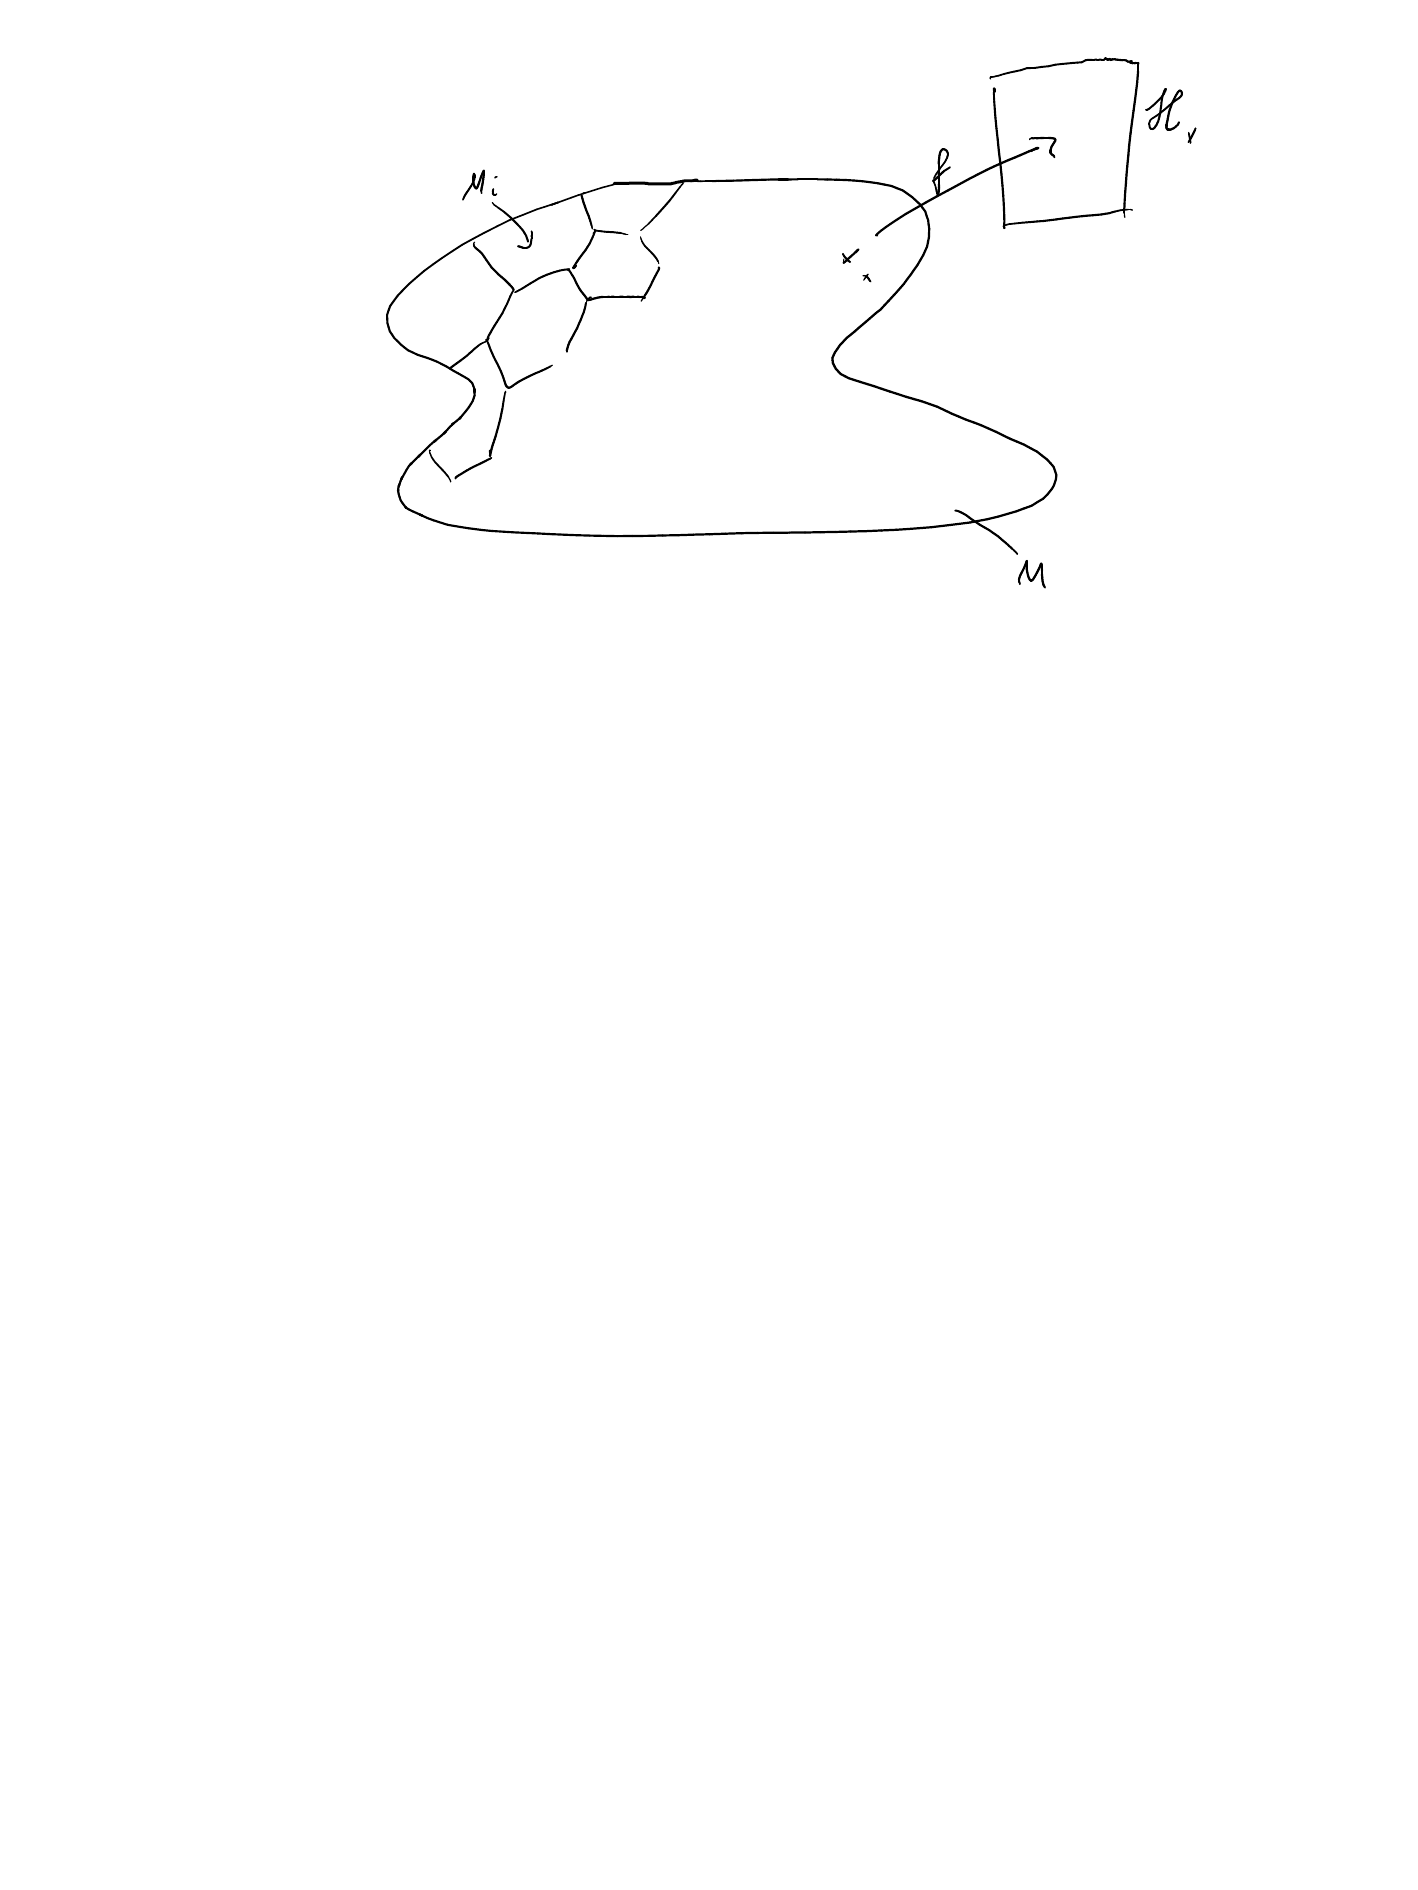
\includegraphics[width=\textwidth]{./direct-integral-graphic-1.png}
  \caption{aa}
  \end{figure}



  % TODO:  (doesn't mention measurablity)

  The next step towards locality is to use two function, by defining
  $L^2(M_1 \sqcup M_2, \mathscr{H}_1 \oplus \mathscr{H}_2)$, where every
  function is defined separately on each $M_i$, and taking values in
  $\mathscr{H}_i$.


  % TODO:  (show the decomp in the fin dim case to make matrix rep clear. and say that the intuition works the same later on)

  Suppose we have a measure space $M$, and for each $x \in M$ a
  Hilbert space $\mathscr{H}_x$ such that $x \mapsto \mathscr{H}_x$ is
  piecewise constant, that is, we have a disjoint decomposition of $M$
  into $\cup_{i=1}^{\infty} M_i$ such that for $x,y \in M_i$,
  $\mathscr{H}_x = \mathscr{H}_y$. 
  % TODO:  (fix with info)
  Interesting aside: the condition that the assignment
  $x \mapsto \mathscr{H}_x$ be piecewise constant is not necessary. We
  can allow the Hilbert spaces to be arbitrary, and in fact uncountably
  infinite. Short answer: magic; slightly less short answer: von Neumann.
  A \emph{section} on $M$ is an assignment $x \mapsto f(x)$, where
  $f(x) \in \mathscr{H}_x$. Since $\mathscr{H}_x$ is piecewise
  constant, the notion of measurability carries over in an obvious manner,
  namely that a measurable function on $M$ is measurable on each $M_i$
  into the appropriate Hilbert space. Let $L^2(M, \{\mathscr{H}_x\})$ be
  the set of square integrable sections $\int \| f \|^2 < \infty$ where
  we identify two sections if they agree almost everywhere. This set is
  then also a Hilbert space with the inner product
  $\langle f | g \rangle = \int_M \langle f(x) | g(x) \rangle$.

  Suppose now we have for each $x \in M$ a unitary representation
  $\pi_x$ of a group $G$ on $\mathscr{H}_x$. We say this is
  measurable when for $g \in G$, $\pi_x(g)$ is a measurable function
  on each $M_i \times G$.

  This allows us to define the relevant representation we intermediately
  care about.

  \begin{rk}[On the notation of the direct integral]
    \label{rem:integral-notation}
    The above notation of $\pi_{\mu, \hilb}$ is generally fine, but putting an
    already hard to read typeface in a small font size into the subscript is
    hard to read. We have introduced it as is to conform with the notation in
    the literature, but in the next section we will encounter a number of
    operations that manipulate these subscripts. For that reason we'll write
    them also in square brackets like so:
    $$
    \pi[\mu, \hilb]
    $$
    meaning the same thing as the subscript notation.
  \end{rk}

  \hypertarget{unitary-representations}{%
  \subsection{Unitary Representations}\label{unitary-representations}}


  % TODO:  (un-garbage intro) We need some more information about
  irreducible unitary representations to understand the action(s) of
  $SL(n, \mathbb{R})$.


%%%%%%%%%%%%%%%%%%%%%%%%%%%%%%%%%%%%%%%%%%%%%%%%%%%%%%%%%%%%%%%%%%%%%%%%%%%%%%%%


\hypertarget{representation-of-rn}{%
\section{Representation of \texorpdfstring{$\bbr^n$}{R\^{}n}}\label{representation-of-rn}}


  \begin{thm}[Zimmer 2.3.3]
    \label{thm:2.3.3}
    \begin{itemize}
      \item For any unitary representation $\pi$ of
        $\mathbb{R}^n$, there exist $\mu, \mathscr{H}_{\lambda}$, on
        $\hat{\mathbb{R}}^n$ such that $\pi \cong \pi_{\mu, \mathscr{H}_{\lambda}}$.
      \item $\pi_{\mu, \mathscr{H}_{\lambda}}$ and
        $\pi_{\mu', \mathscr{H}_{\lambda}'}$ are unitarily equivalent if and only if 
        \begin{itemize}
          \item $\mu \sim \mu'$, i.e., they are in the same measure class
          \item and $dim\mathscr{H}_{\lambda} = dim \mathscr{H}_{\lambda}'$ a.e.
        \end{itemize}
    \end{itemize}
  \end{thm}

  \begin{pf}
    \label{pf2.3.3}
  \end{pf}

  \begin{thm}[Zimmer 2.3.4]
    \label{thm:2.3.4}
    Let $\pi = \pi_{\mu, \hilb_{\lambda}}$, $A\in  \Aut(\bbr^n)$, $\alpha$ the
    adjoint automorphism of $\hat{\bbr}^n$. Then
    \begin{itemize}
      \item $\alpha(\pi)$ is unitarily equivalent to $\pi[\alpha_*\mu]$
    \end{itemize}
  \end{thm}

  \begin{pf}
    \label{pf:2.3.4}
  \end{pf}

  \begin{thm}[Zimmer 2.3.5, from \Citeauthor{mackey76} \cite{mackey76}]
    \label{thm:2.3.5}
    Suppose $\mathbb{R}^n \subset G$ is a normal subgroup and $\pi$ is a unitary representation of $G$.
    Write $\pi | \mathbb{R}^n \cong \pi_{(\mu, \mathscr{H}_{\lambda})}$ for some
    $(\mu, \mathscr{H}_{\lambda})$ by 2.3.3. Then  
    \begin{itemize}
      \item $\mu$ is quasi-invariant under the action of $G$ on $\hat{\mathbb{R}}^n$. 
      \item If $E \subset \mathbb{R}^n$ is measurable, let
        $\mathscr{H}_E = L^2(E, \mu, \{\mathscr{H}_{\lambda}\})$.
        Then $\pi(g)\mathscr{H}_E = \mathscr{H}_{g \cdot E}$
      \item If $\pi$ is irreducible, then $\mu$ is ergodic and $dim\mathscr{H}_{\lambda}$ is
        constant on a $\mu$-conull set.
    \end{itemize}
  \end{thm}

  \begin{pf}
    % TODO: finish proof lmao
  \end{pf}

  % TODO: this was planted here so I could refer to it later on.
  \begin{thm}[Zimmer 2.3.6]
    \label{thm:2.3.6}
    Let \mpi be  a unitary representation of $P = AN$.
    \begin{itemize}
      \item either $\pi|N$ has non-trivial invariant vectors or
      \item or for $g \in A$ and any vectors, $v$, $w$, the matrix coefficients
        $\langle \pi(g)v, w \rangle \rightarrow 0$ as $g \rightarrow \infty$.
    \end{itemize}
  \end{thm}

  \begin{pf}
    We identify $N$ with \bbr via the map $\ipmatrix{1 & x \\ 0 & 1} \mapsto x$ 
     % TODO: fill in
  \end{pf}


  % TODO:  (this drops out of nowhere) -> schur decomp
  % TODO: Schur decomp
  All the irreducible unitary
  representations of $\mathbb{R}^n$ are one-dimensional.

  It turns out that the group unitary representations on $\mathbb{R}^n$
  are isomorphic to $\mathbb{R}^n$. So we define a map from
  $\mathbb{R}^n$ to $\mathcal{U}(\mathbb{C})$ and show that it's in
  fact bijective. Let $\theta$. $t$ be in $\mathbb{R}^n$ and let
  $\lambda_{\theta}(t) = e^{i\langle \theta | t \rangle}$. This is in
  fact a unitary automorphism on $\mathbb{C}$ by multiplication. To
  clarify, for every $\theta \in \mathbb{R}^n$ we have a representation
  given by
  \begin{align*}
    \lambda_{\theta}:\ & \mathbb{R}^n \rightarrow \mathcal{U}(\mathbb{C}) \\
    & t \mapsto e^{i \langle \theta | t \rangle}
  \end{align*}
  We denote the group of representations by $\hat{\mathbb{R}}^n$. It
  is in fact a group under pointwise multiplication.


  % TODO:  (this sort of drops out of nowhere)
  This definition is maybe a bit dense, so here is the assignment formatted in
  pseudo code. This might help some reader more familiar with programming than
  mathematics. The more mathematically inclined may ignore it. It is not
  relevant other than to further the understanding of the above definition.
  Note here that $\text{lambda}$ denotes the programming term of a lambda
  function, an unfortunate notation collision.
  \begin{align*}
  & \text{func }\ \pi_{\mu,\mathscr{H}_{\lambda}}(t: \mathbb{R}^n) \rightarrow \mathcal{U}(L^2(\hat{\mathbb{R}}^n)) \ \{ \\
  & \qquad \text{return lambda}(f:\ L^2(\hat{\mathbb{R}}^n)) \rightarrow L^2(\hat{\mathbb{R}}^n) \ \{ \\
  & \qquad \qquad \text{return lambda}(\lambda:\ \hat{\mathbb{R}}^n) \rightarrow \mathscr{H}_{\lambda} \ \{ \\
  & \qquad \qquad \qquad \text{return }\lambda(t)f(\lambda) \\
  & \qquad \qquad \} \\
  & \qquad \} \\
  & \} \\
  \end{align*}

  \hypertarget{the-connection-between-ergodicity-and-unitary-representations}{%
  \subsection{The Connection between Ergodicity and Unitary Representations}\label{the-connection-between-ergodicity-and-unitary-representations}}

  approach: - char func - char func in L2(S) and non-trivial - if A
  invariant then char func invariant as a vector in L2(S) - due diligence:
  make sure measure works

  To see why we care about unitary representations at all if we really
  want ergodicity, we neeedd to make the folllowing connection. We use the
  characteristic function of a set to connect the set to a vector in
  $L^2(S)$. The characteristic function of a subset $A\subset S$, is
  defined as $\chi_A(x) = 1$ for $x \in A$ and $0$ otherwise.

  This representation allows us to pass from talking about sets to talking
  about vectors, while retaining the properties we care about.

  \begin{thm}[Zimmer 2.2.17]
    \label{thm:2.2.17}
    An action $G\curvearrowright S$, with **finite** invariant measure is ergodic
    on $S$ if and only if the restriction of the above representation to  in
    $L^2(S) \ominus \mathbb{C}$ has no invariant vectors.
  \end{thm}
    
  Since $S$ has finite measure, assume $\mu(S) =1$.

  \begin{pf}
    "$\Leftarrow$": Proof by contrapositive: If $A\subset S$ is $G$-invariant
    with measure $0 < \mu(A) < \mu(S) = 1$ then $\chi_A$ is also $G$-invariant
    in $L^2(S)$ as well as the projection $\chi_A - \mu(A)\cdot 1$ in
    $L^2(S)\ominus \mathbb{C}$. Therefore there exists an invariant vector in
    $L^2(S)\ominus \mathbb{C}$. "$\Rightarrow$": (\cite{Kerr16}(Prop 2.7))
    Suppose the action is ergodic and $f\in L^2(S)\ominus \mathbb{C}$ is
    $G$-invariant. We can find a measurable set $D\subset \mathbb{C}$ such that
    $0<\mu(f^{-1}(D)) < 1$ and denote $\widetilde{A} = f^{-1}$. Now we verify
    ergodicity. For every $g\in G$ the symmetric difference $g\widetilde{A}
    \Delta \widetilde{A}$, for which all points are in the set $\{x \in X | \
    |f(x)-sf(x)| > 0\}$, which has measure zero because $\|f- sf\|_2=0$.
    Therefore the action fails to be ergodic.
  \end{pf}

  The adjective ``finite'' on the measure is necessary, because for a set
  $A$ of infinite measure the statement is no longer true as $\chi_A$
  will no longer be in $L^2$.

  % TODO: This is of course fine, because we care about the special case where the space $S$ in question is the quotient of a lattice $G/\Gamma$, which has finite measure by definiton. So this restriction is not only acceptable but desired.

  If $A\subset S$ is $G$-invariant then $\chi_A\in L^2(S)$ will also
  be $G$-invariant. 
  % TODO:  (is ominus actually a valid op here? yes, see Kerr Li prop 2.7)
  For $A$ neither null nor conull then
  $\chi_A$, $f_A \neq 0$, where $f_A$ is the projection of
  $\chi_A$ onto $L^2(S) \ominus \mathbb{C}$.


%%%%%%%%%%%%%%%%%%%%%%%%%%%%%%%%%%%%%%%%%%%%%%%%%%%%%%%%%%%%%%%%%%%%%%%%%%%%%%%%


\hypertarget{proof-for-sl2r}{%
\section{Proof for \texorpdfstring{$SL(2, \mathbb{R})$}{SL(2, R)}}\label{proof-for-sl2r}}


  We start here because it is an easy example of the theorem and a general
  group $G$ has many subgroups locally isomorphic to
  $SL(2, \mathbb{R})$. Later we extend the proof, first to
  $SL(n, \mathbb{R})$ and then to a general $G$.

  To state our intentions: we first show that either the matrix
  coefficients vanish as we want, or there exist invariant vectors. Then
  we show that there are no invariant vectors, completing the statement.

  We're going to use the following decomposition, which we take for
  granted 
  % TODO:  (find reference for Iwasawa decomposition).
  The so called Iwasawa decomposition of $SL(2, \mathbb{R})$ into three
  matrices $K$, $A$, and $N$, defined as
  \begin{align}
  K & =\quad \left\{ \begin{pmatrix} \cos\theta & -\sin\theta \\ \sin\theta & \cos\theta\end{pmatrix} \subset SL(2, \mathbb{R})  \ | \ \theta \in \mathbb{R} \right\} \\
  A & =\quad \left\{ \begin{pmatrix} r & 0 \\ 0 & r^{-1} \end{pmatrix} \subset SL(2, \mathbb{R})  \ | \ r > 0 \right\} \\
  N & =\quad \left\{ \begin{pmatrix} 1 & x \\ 0 & 1 \end{pmatrix} \subset SL(2, \mathbb{R})  \ | \ x \in \mathbb{R} \right\}\\
  \end{align}


  \hypertarget{theorem-for-p}{%
  \subsection{Theorem for \texorpdfstring{$P$}{P}}\label{theorem-for-p}}

  \begin{lem}[decomposition of \sltr and $P$]
    \label{ref:lem:decomp}
    \begin{enumerate}
      \item The upper triangular group $P$ and $\bar{P}$ generate \sltr.
      \item The upper triangular group can be decomposed into the semidirect product:
        $$
        P = AN = \begin{pmatrix}a & 0 \\ 0 & a^{-1}\end{pmatrix} \begin{pmatrix}1 & b \\ 0 & 1\end{pmatrix}
        $$
      \item $N$ is normal in $P$
    \end{enumerate}
     
  \end{lem}

  \begin{pf}
    \label{ref:lem:pf:decomp}
    We look at the subgroup
    \[P \subset SL(2, \mathbb{R}) = \begin{pmatrix}a & b \\ 0 & a^{-1}\end{pmatrix}\]
    of upper triangular matrices. Together with the lower diagonal matrices
    $\bar{P}$, they generate $SL(2, \mathbb{R})$. To see this, decompose
    as follows: \[\begin{pmatrix}1&0\\\alpha&1\end{pmatrix}
    \begin{pmatrix}x&0\\0&1/x\end{pmatrix}
    \begin{pmatrix}1&\beta\\0&1\end{pmatrix} = 
    \begin{pmatrix} x&\beta x\\\alpha x& \alpha\beta x+1/x\end{pmatrix}\]
    For any matrix $A = \begin{pmatrix}a & b \\ c & d\end{pmatrix}$ in
    $SL(2, \mathbb{R})$ with matrix coefficient $a \neq 0$, we can solve
    for $x,\alpha, \beta$. In the case of $a = 0$ we can use the
    following construction:
    \[
      \begin{pmatrix} 1&0\\\alpha&1\end{pmatrix}
      \begin{pmatrix} 1&\beta\\0&1\end{pmatrix}
      \begin{pmatrix} 1&0\\\gamma&1\end{pmatrix}
      \begin{pmatrix} 1&\delta\\0&1\end{pmatrix}=
      \begin{pmatrix}
        1+\beta\gamma&\delta(1+\beta\gamma)+\beta\\
        \alpha(1+\beta\gamma)+\gamma&\alpha\delta(1+\beta\gamma)+\alpha\beta+\gamma\delta+1
      \end{pmatrix}
    \]
    If $1 + \beta\gamma = 0$, the above product becomes
    $\begin{pmatrix} 0&\beta\\ \gamma& 1+\alpha\beta+\gamma\delta \end{pmatrix}$
    and we can make suitable choices for $\alpha, \beta, \gamma, \delta$
    to construct $A$.

    Note first, that $N$ is normal in $P$. To see this, first calculate that the
    inverse of a matrix $\ipmatrix{ a & x \\ 0 & a^{-1} }$ in $P$ is $\ipmatrix{
    a^{-1} & -x \\ 0 & a }$. Next note that the result of conjugation with an
    element in $P$ is again in $N$: $\ipmatrix{ a & x \\ 0 & a^{-1} } \ipmatrix{1 &
    y \\ 0 & 1} \ipmatrix{ a^{-1} & -x \\ 0 & a } = \ipmatrix{1 & a^2x \\ 0 & 1}$.
    This defines a group action $P \curvearrowright N \rightarrow N$ by
    multiplication with $a^2$.
  \end{pf}


  % TODO: various decompositions for how we want to look at sl2r for 

  \hypertarget{theorem-for-cartan-decomposition}{%
  \subsection{Theorem for Cartan
  decomposition}\label{theorem-for-cartan-decomposition}}

  \hypertarget{polar-decomposition-to-cartan}{%
  \subsection{Polar decomposition to Cartan}
  \label{polar-decomposition-to-cartan}}

  $T = US$ for some unitary $U$ and a sym pos def $S$. $S$ can be
  diagonalized into $U_0 D U_0^{-1}$ so we can write
  $T = U U_0 D U_0^{-1} = U_1 D U_2$ for $U_i \in SO(2, \mathbb{R})$.
  Then $SL(2, \mathbb{R}) = KAK$ for $K = SO_2$ and $A$ the diagonal
  group. This is the Cartan decomposition.





  \begin{lem}
    \label{lemma}
    If $\pi$ is a unitary representation of a Group $G$ (which is assumed to be second countable) and we can write $G =
    KAK$, with $K$ compact, then it suffices to check that the matrix
    coefficients vanish on A as $g \rightarrow \infty$.
  \end{lem}

  \begin{pf}
    \label{pf:lemma}
    We take vectors $v, w$ and write $g \in G$ as $g = k_1 a k_2$.
    Then the corresponding matrix
    coefficient can be written as $\langle \pi(g)v|w \rangle = \langle \pi(a) \pi(k_2) v | \pi(k_1)^{-1} w \rangle$.

    We make a proof via contraposition.
    If there exists a matrix coefficient that fails to vanish as $g \rightarrow \infty$
    we can find a sequence $g_n = k_{1,n} g_{n} k_{2,n} \rightarrow \infty$ as
    $n \rightarrow \infty$ with
    $|\langle \pi(g_n) v | w \rangle | \geq \varepsilon$ for some $\varepsilon > 0$.

    Because $G$, and therefore $K$ is second countable and compact, it is also sequentially compact.
    So we can suppose $k_{1,n} \rightarrow k$ and $k_{2,n}^{-1} \rightarrow k'$.
    Then, for $n$ sufficiently large, $|\langle \pi(a_n)\pi(k)v | \pi(k') w \rangle | \geq \varepsilon/2$.
    This follows from the following estimation, where we ommit the representation $\pi$ for legibility:

    \begin{align*}
        &=\abs{\inn{a_n k_n v, k_n' w} - \inn{a_n k v, k' w}} \\
        &= \abs{\inn{a_nk_nv - a_nkv, k_n'w} \ + \ \inn{a_nkv, k_n'w - k'w}}  \\
        &\leq \abs{\inn{a_nk_nv - a_nkv, k_n'w}} \ + \ \abs{\inn{a_nkv, k_n'w - k'w}} \quad \text{Triangle Inequality} \\
        &\leq \norm{a_nk_nv - a_nkv}\norm{k_n'v} \ + \ \norm{a_nkv}\norm{k_n'w - k'w} \quad \text{Cauchy-Schwarz} \\
     \end{align*}

    From here, we can pick an $n$ large enough to assert the inequality.

    But since $K$ is compact and $g_n \rightarrow \infty$, we must have
    $a_n \rightarrow \infty$. This shows that the must be a matrix
    coefficient in $\pi | A$ that fails to vanish at infinity.
  \end{pf}



%%%%%%%%%%%%%%%%%%%%%%%%%%%%%%%%%%%%%%%%%%%%%%%%%%%%%%%%%%%%%%%%%%%%%%%%%%%%%%%%

\hypertarget{proof-for-slnr}{%
  \section{Proof for \texorpdfstring{$SL(n, \mathbb{R})$}{SL(n, R)}}
\label{proof-for-slnr}}


% old stuff

  \hypertarget{theorem-for-sl2-r}{%
    \subsection{Theorem for \texorpdfstring{$SL(2, \mathbb{R})$}{SN(2, R)})}\label{theorem-for-sl2-r}}

  If $\pi$ is a unitary representation of $G = SL(2, \mathbb{R})$ with no
  invariant vectors, then all matrix coefficients of $\pi$ vanish at $\infty$.


  We can now start on the statement for \sltr. Thanks to the work we did in the
  preceeding chapter, the statement is actually not very difficult to prove. The
  theorem \ref{thm:2.3.6} and the preceeding lemma \ref{lemma} does the bulk of
  the heavy lifting here.


  \begin{pf}
    By assumption, \G has no invariant vectors. By theorem \ref{thm:2.3.6},
    There are two possible cases. Either $N$ has non-zero invariant vectors,
    or the matrix coefficients vanish along $A$.

    Should there be no non-zero invariant vectors, as we'll show, then
    the matrix coefficients vanish along $A$, and, by lemma \ref{lemma},
    vanishing along $A$ implies vanishing along \G.

    To see that there are no $N$-invariant vectors, we assume towards a contradiction
    that there are $N$-invariant vectors and show that these must be \G-invariant as well,
    which contradicts our assumption.

    Suppose there is a vector $v$ that is \Ninv, meaning $\pi(n)v = v$ for all $n \in N$.
    As a shorthand, define the function $f(g) = \langle \pi(g)v,v\rangle$.
    This defines a continuous bi-\Ninv function on $G$.

    This is because $f(gn) = \langle \pi(gn)v,v,\rangle = \langle \pi(g)\pi(n)v,v\rangle = \langle \pi(g)v,v\rangle = f(g)$,
    and $f(ng) = \langle \pi(n)\pi(g)v,v\rangle \xrightarrow{unitary} \langle \pi(g)v, \pi(n)^{-1}v\rangle = f(g)$.

    Thus $f$ lifts from a continuous bi-\Ninv function on $G/N$.

    \G acts transitively on $\bbr^2\setminus \{0\}$ by matrix multiplication,
    and, using the fact that $N$ is exactly the stabilizer of $\ipmatrix{1 \\
    0}$, we get an isomorphism $G/N \cong \bbr^2\setminus \{0\}$ \footnote{This
    is due to the fact that for a transitive action $G\curvearrowright X$ there
    is an isomorphism $G/Stab_G(x) \rightarrow X$ sending $g\cdot Stab_G(x)
    \mapsto gx$.}.

    Calculating the orbits of this action we have $\ipmatrix{1 & x \\ 0 &
    1}\ipmatrix{a \\ b} = \ipmatrix{a +bx \\ b}$. So there exist two kinds of
    orbits: for $b \neq 0$. the orbit is the horizontal line at height $b$ and
    for $b=0$ every individual point $(a\ 0)$ on the $x$-axix. (See Figure~\ref{fig:n-orbits-in-r2}). As $f$ is \Ninv,
    $f$ will be constant along these orbits. Because $f$ is continuous, $f$ will
    also be constant along the $x$-axis.

    \begin{figure}
      \begin{center}
        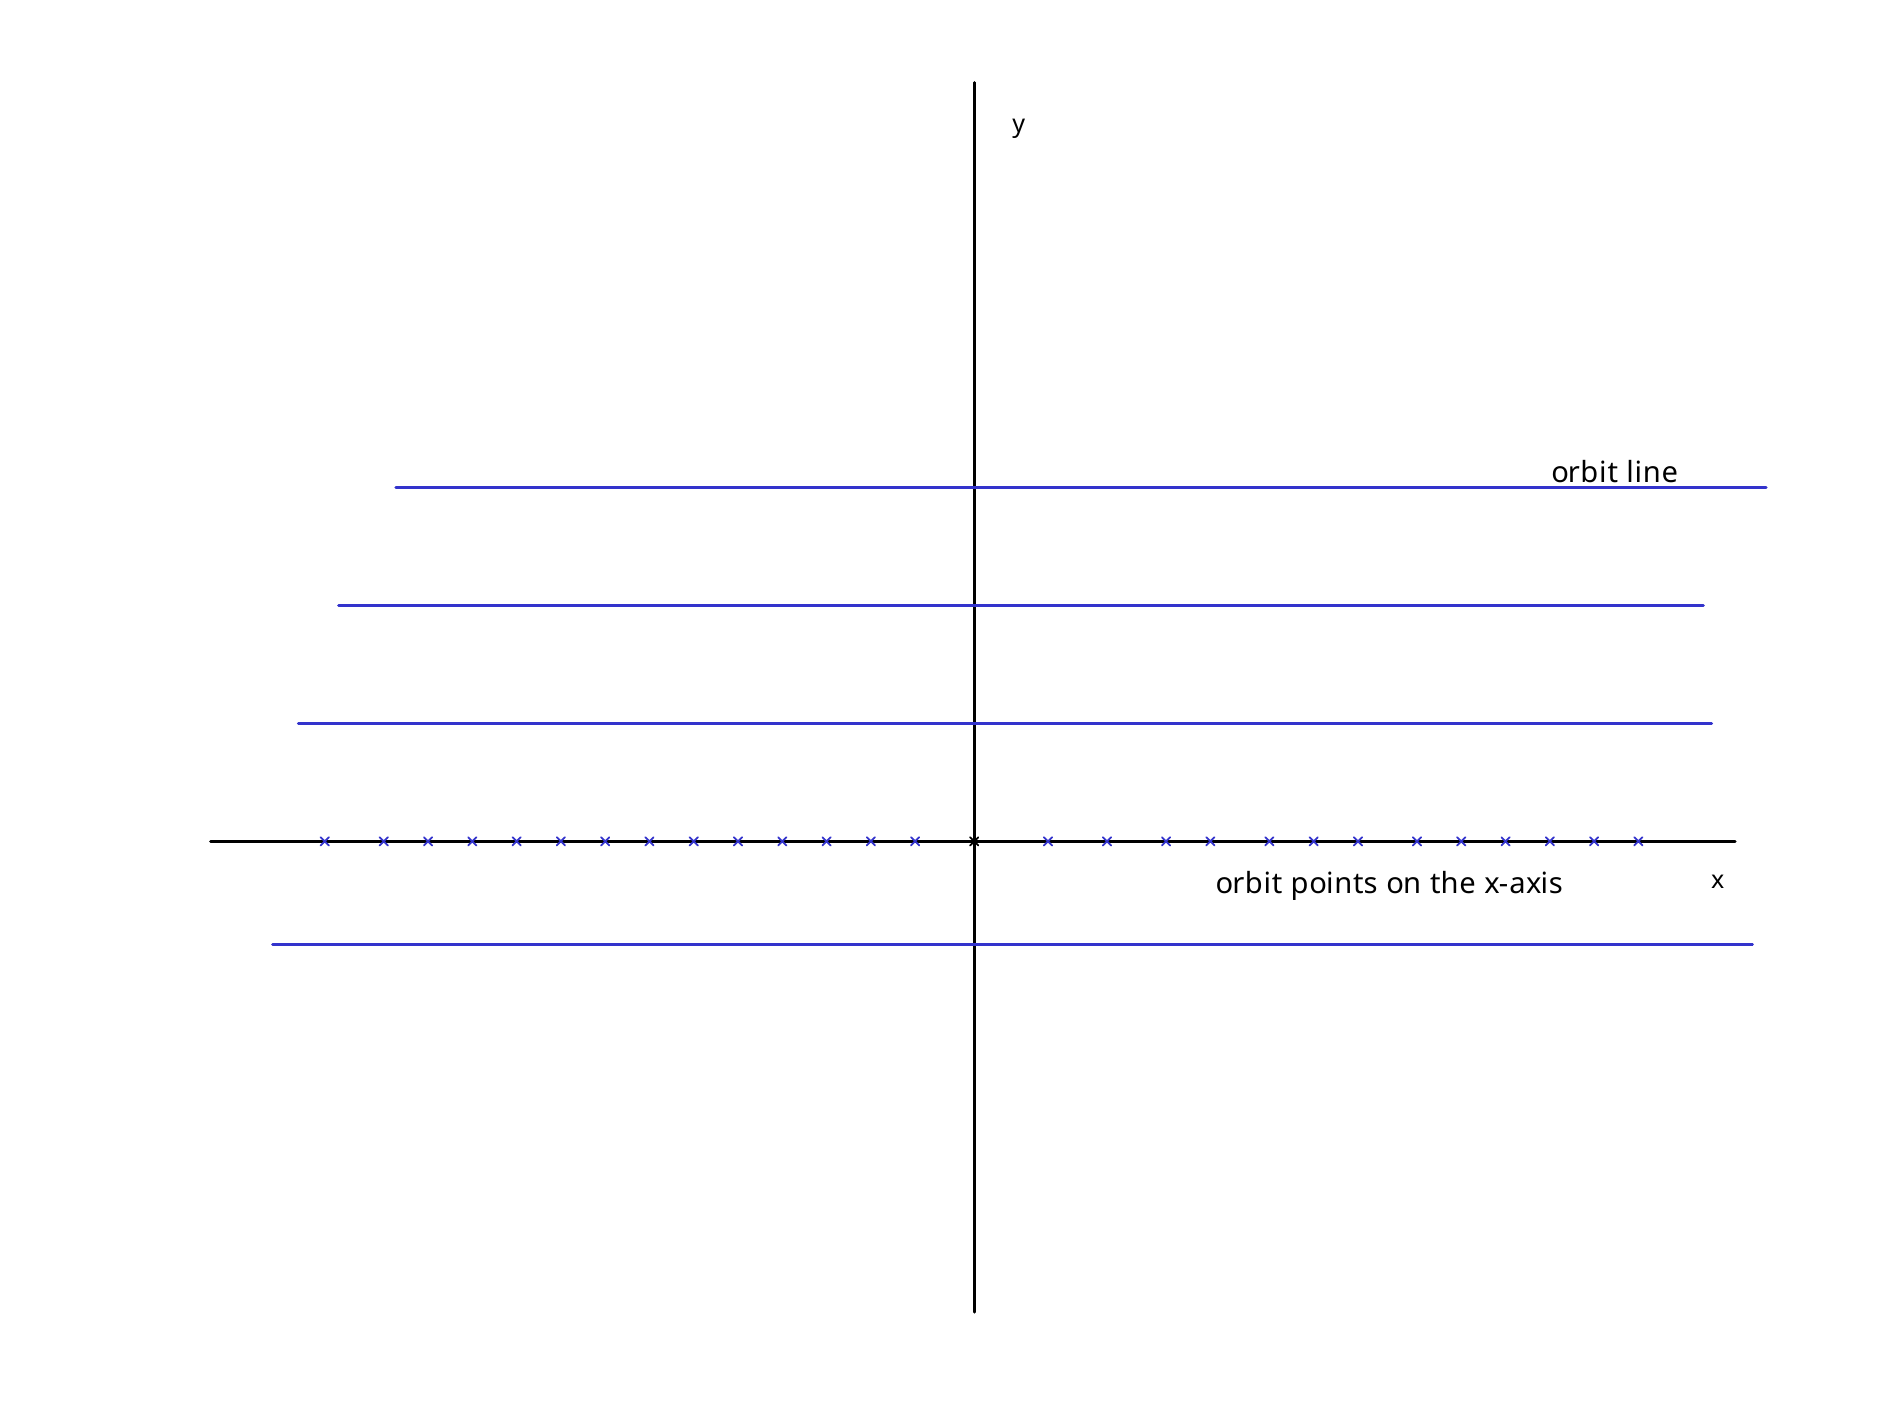
\includegraphics[width=0.95\textwidth]{N-orbits-in-R2-1.png}
      \end{center}
      \caption{The orbits of $N$ on $G/N$ correspond either to the horizontal lines parallel to the x-axis or to the individual points on the x-axis. }
      \label{fig:n-orbits-in-r2}
    \end{figure}

    But we can also identify the $x$-axis with $P/N$ by $\ipmatrix{a & b \\ 0 &
    a^{-1}}\ipmatrix{x \\ 0} = \ipmatrix{ax \\ 0}$. Therefore $f$ is also
    constant on $P$. So it follows that $v$ is $P$-invariant. And as we've seen
    in the \hyperref[sec:introduction]{intoduction}, we can identify $G/P$ with
    the real projective line and $P$ has a dense orbit in $G/P$ so $f$ is
    constant on $G$ and therefore $v$ is actually \G-invariant, contradicting our
    assumption.
  \end{pf}


%%


  In this section we'll prove the statement for $G = \slnr$ and later show how
  the proof is extended to a general group \G. We begin just as for \sltr, by
  applying \hyperref[lemma]{lemma} \ref{lemma}. Thus it suffices to show that
  matrix coefficients vanish on $A \subset G$ to imply that they vanish on \G.


  \begin{math}
    \begin{pmatrix}
      1 & b_{1,2} & & \cdots & & b_{1,n} \\
      0 & & &  & \\
      \vdots & & & \Id_{n-1} & \\
      0 & & & & \\
    \end{pmatrix}
  \end{math}

  Note: in the case of $n = 2$, which reduces this to \sltr and the above matrix to $N$ from the previous proof.





  % TODO: unoriginal
   Following our remark in the preface, we shall
  prove this in detail for G = SL(n, IR), and then indicate how the proof
  carries over to general G. Let A c SL(n, IR) be the group of diagonal
  matrices. We denote an element aEA by (at, \ldots{} , an), where these
  are to be interpreted as the diagonal elements of a matrix. We note Ila;
  = 1. Let B be the set of matrices (cii) with cu = 1, and cii = 0 fori
  =f.~j and i \textasciitilde{} 2. We denote an element bEB by b = (1, b 2
  , •.• , bn) where this is to be interpreted as the first row of the
  corresponding matrix. Then30 Ergodic theory and semisimple groups aBa- 1
  = B for aEA, and hence H = AB is a subgroup of G, and B c H is normal.
  We observe B \textasciitilde{} IRn- 1 . As with SL(2, IR), by Lemma
  2.4.1, it suffices to show that the matrix coefficients of n: IA vanish
  at oo. For SL(2, IR) we obtained this using knowledge of the
  representation of P. In our more general situation, we will examine the
  representation of H. (Note that H = P for n = 2.) Express n: IB
  \textasciitilde{} n:\textless\textasciitilde.x .) (by 2.3.3) via the
  above identification of B with IRn- 1 . Matrix multiplication shows that
  for aEA, bEB, aba- 1 = (1, a 1 ai 1 b2, \ldots{} , a 1 a;; 1 bn)EB. The
  adjoint action on !Rn- 1 will be given by the same expression, replacing
  b; by the dual variables h i = 2, \ldots{} , n.~Therefore, if E, F c
  !Rn- 1 are compact subsets which are disjoint from the union of the
  hyperplanes ).; = 0, i = 2, \ldots{} , n then for aEA outside a
  sufficiently large compact set, we have a· En F = 0. Therefore, arguing
  exactly as in the proof of Theorem 2.3.6, we deduce that if f.J. assigns
  measure 0 to the union of the hyperplanes A.; = 0, then all matrix
  coefficients vanish along A, and by our comments above, this suffices to
  prove the theorem. Therefore, it remains to show that f.J.(\{A.; = 0\})
  \textgreater{} 0 is impossible. If f.J.(\{J.; = 0\}) \textgreater{} 0,
  then by definition of f.J.\textless{} 11 .x,J, the subgroup B; c B, B; =
  \{bEBibi = 0 fori \#j\} leaves non-trivial vectors invariant (namely,
  the subspace .\#p.;=o 1.) However B; c H; c G where H; \textasciitilde{}
  SL(2, IR) and is defined as follows H; = \{(cik)ESL(n, IR)Icjj = 1 for j
  \# 1, i, and for j \# k and \{1, i\} \# \{j, k\}, Cjk = 0\}. From the
  vanishing of matrix coefficients for SL(2, IR), (2.4.2), the existence
  of a B;-invariant vector implies the existence of a H;-invariant vector
  (since B; is clearly non-compact). In particular, A;= H; n A has
  non-trivial invariant vectors. Let W= \{vEYl'ln:(a)v =
  vforallaEA;\}.Itsufficestoshowthat WisG-invariant. For then the
  representation n:w ofG on Whas kernel (n:w) ::::J A; which by simplicity
  of G implies that kernel(n:w) = G, so that G itself leaves all vectors
  in W fixed, contradicting our assumptions. (For the analogous argument
  in the semisimple case the fact that dim(kernel n:w) \textgreater{} 0
  contradicts the assumption that no simple factor of G leaves vectors
  invariant.) We now turn to G-invariance of W. For k \# j, let Bki c G be
  the one- dimensional subgroup defined by Bki = \{(c,.)lc,, = 1, and for
  r \#sand (r, s) \# (k, j), c,. = 0\}. We consider two possibilities. (i)
  k \# i or 1 andj \# i or 1. Then Bki commutes with A;, and hence Bki
  leaves W invariant. (ii) If \{ k, j\} n \{ i, 1\} \# 0 then A;
  normalizes Bki· Hence A;Bki is a 2-dimensional subgroup and is
  isomorphic to P in such a way that A;+-+(diagonal matricesMoore's
  ergodicity theorem 31 in P), Bki- N. By Corollary 2.3.7, all
  A;-invariant vectors are also Bki invariant. Hence in this case, too,
  Bki leaves W invariant. Finally, we remark that since A; c A, A abelian,
  A also leaves W invariant. However, A and all Bki together generate G.
  Therefore G leaves W invariant, completing the proof.


%%%%%%%%%%%%%%%%%%%%%%%%%%%%%%%%%%%%%%%%%%%%%%%%%%%%%%%%%%%%%%%%%%%%%%%%%%%%%%%%


\hypertarget{proof-for-a-general-G}{%
\section{Proof for a general \texorpdfstring{$G$}{G}}\label{proof-for-a-general-G}}


  % TODO: unoriginal
   In concluding this section, we indicate the
  modifications necessary in the above argument for a general semisimple
  G. Let A c G be a maximal IR-split torus. Then A c G' c G where G' is
  semisimple and split over IR, and A is the maximal IR-split torus of G'.
  Choose a maximal linearly independent set S of positive roots of G'
  relative to A such that for a, \{3ES, a+ \{3 is not a root. Then the
  direct sum of the root spaces is the Lie algebra of an abelian subgroup
  B c G', with dim B =dim A, and B is normalized by A. The representations
  of AB can be analyzed exactly as in the case of SL(n, IR), and since the
  relevant copies of s1(2, IR) are present, we deduce that either we are
  done, or some one-dimensional subgroup A 0 c A leaves a non-trivial
  vector fixed. (Actually to obtain this we may need to use the universal
  covering G of SL(2, IR) rather than SL(2, IR) itself. Namely, we need
  that for N c SL(2, IR) as in the proof of2.4.2, N c G the connected
  component of the lift of N to G (so that N \textasciitilde{} N ), that N
  invariant vectors are G-invariant. However, this follows by elementary
  covering space arguments applied to the picture in the proof of 2.4.2.
  If G is algebraic, which will be our main concern, consideration of
  SL(2, IR) suffices.) The proof then proceeds as in the case of SL(n,
  IR); G is generated by elements that either commute with Ao or lie in a
  suitable copy of the group P.


%%%%%%%%%%%%%%%%%%%%%%%%%%%%%%%%%%%%%%%%%%%%%%%%%%%%%%%%%%%%%%%%%%%%%%%%%%%%%%%%


\hypertarget{outro}{%
\section{Outro}\label{outro}}


  Now that we've proven the theorem, it's natural to ask what we do with it now.
  At first glance, the statement about matrix coefficients doesn't seem particularly useful,
  but recall from this \hyperref[the-connection-between-ergodicity-and-unitary-representations]{section}
  that we have a connection to invariant subsets of a possibly ergodic space.

  We have mentioned in the very beginning where we wanted to go with this, but let's recall it here.

  The problem we posed at the beginning of the paper is the following:

  \begin{problem}[When do closed subgroups act ergodically]
    Let \G be a semisimple Lie group and $S$ an ergodic \G-space. If $H\subset G$ is a closed subgroup, when is $H$ ergodic on $S$.
  \end{problem}

  \begin{thm}[Zimmer 2.2.19, originally \citeauthor{Moore66}\cite{Moore66}]
    \label{thm:2.2.19}
     Let $G_i$ be semisimple, non-compact Lie groups and $G = \prod G_i$ and
     suppose \mpi is a unitary representation that has no invariant vectors of
     \G such that \mpi has no invariant vectors for each $\pi|G_i$. If $H
     \subset G$ is a closed subgroup and $\pi|H$ has non-trivial invariant
     vectors then $H$ is compact.
  \end{thm}

  \begin{pf}
     % TODO: fill in
  \end{pf}


  % TODO: for the case of spaces with finite invariant measure the established condition is exactly necessary and sufficient for ergodicity.
  \hyperref[thm:2.2.17]{invariant vec}

  % TODO: Recall that the defition of a lattice specifies that the quotient $G/Gamma$ has finite measure. This means for actions on that space, searching for invariant vectors is exactly equivalent to establishing ergodicity.

  % lemma 2.2.13
  % leads to thm 2.2.15
  % leads to thm 2.2.6 Moore's ergodicity theorem. find reference

  \begin{thm}[Zimmer 2.2.15]
    \label{thm:2.2.15}
     
  \end{thm}

  \begin{pf}
     
  \end{pf}

  \begin{thm}[Zimmer 2.2.6, Moore's Ergodicity Theorem]
    \label{thm:2.2.6}
    \G as usual.
    Let $\Gamma \subset G$ be an irreducible Lattice. % TODO: irreducible?
    If $H \subset G$ is a closed subgroup and $H$ is not compact, then $H$ is ergodic on $G/\Gamma$
  \end{thm}

  \begin{pf}
     
  \end{pf}

  % TODO: cor 2.2.4

  % TODO: mat coeff vanish > no invv means H cpct > no invv iff H erg in L^2 - C > H closed non-cpct impl H erg > S=G/Gamma > original problem


  \hypertarget{return-of-the-initial-example}{%
  \subsection{The return of the initial example
  }\label{return-of-the-initial-example}}


  Looking back at the initial example, the case becomes clear.
  applying the \hyperref{thm:}[theorem] with $\G = \sltr$.
  A lattice \Gamm in \G acts ergodically on $\bar{\bbr}$, since $\bar{\bbr} \cong \sltr / P$ and $P$ is not compact. %% Ex 2.2.8

  % TODO: def 2.2.4 needs to get in here somehow.

  % circle back to fractional linear transforms.
  % hyperbolas! 3 cases comp eucl and non-comp. if we want to go to infinity
  % and don't want boring examples, hyperbolic geometry is necessary.
  % fractional linear transforms. riemann sphere model?


%%%%%%%%%%%%%%%%%%%%%%%%%%%%%%%%%%%%%%%%%%%%%%%%%%%%%%%%%%%%%%%%%%%%%%%%%%%%%%%%



\cleardoublepage

\appendix

\hypertarget{auxilliary-statements}{%
\section{Auxilliary Statements}\label{auxilliary-statements}}

\begin{prop}
  In a second countable topological space, compactness and sequential compactness are equivalent.
\end{prop}

\begin{pf}
  no proof % TODO: where??
\end{pf}

\section{List of Theorems}
\theoremlisttype{allname}
\listtheorems{thm,lem}

\phantomsection
\addcontentsline{toc}{section}{List of Figures}
\listoffigures

\phantomsection
\addcontentsline{toc}{section}{Bibliography}
\printbibliography

\end{document}
